\chapter{Central Processing Units}\label{ch14}
\section{Introduction}

One of the important benefits of using a simulator like \Le is that a circuit designer can simulate digital systems to determine logic flaws or weaknesses that must be addressed before a physical \gls{ic} is manufactured. This chapter introduces the concept of simulation and includes several examples of simulated systems.

%***************************************************************************
% Section: CPU
%***************************************************************************
\section{Central Processing Unit}
\label{SIM:sec:cpu}

\subsection{Introduction}
\label{SIM:subsec:intro_to_cpu}

The \gls{cpu} is the core of any computer, tablet, phone, or other computer-like device. While many definitions of \gls{cpu} have been offered, many quite poetic (like the ``heart'' or ``brain'' of a computer); probably the best definition is that the \gls{cpu} is the intersection of software and hardware. The \gls{cpu} contains circuitry that converts the ones and zeros that are stored in memory (a ``program'') into controlling signals for hardware devices. The \gls{cpu} retrieves and analyzes bytes that are contained in a program, turns on or off multiplexers and control buffers so data are moved to or from various devices in the computer, and permits humans to use a computer for intellectual work. In its simplest form, a \gls{cpu} does nothing more than fetch a list of instructions from memory and then execute those instructions one at a time. This chapter explores \glspl{cpu} from a theoretical perspective.

\subsubsection{Concepts}

A \gls{cpu} processes a string of ones and zeros and uses the information in that binary code to enable/disable circuits or hardware devices in a computer system. For example, a \gls{cpu} may execute a binary code and create electronic signals that first place data on the computer's data bus and then spins up the hard drive to store that data. As another example, perhaps the \gls{cpu} detects a key press on a keyboard, transfers that key's code to memory and also sends a code to the monitor where specific pixels are activated to display the letter pressed.

Figure \ref{sim:fig:simple_data_flow_control_circuit} illustrates a very simple circuit used to control the flow of data on a data bus.

\begin{figure}[H]
  \caption{Simple Data Flow Control Circuit}
  \label{sim:fig:simple_data_flow_control_circuit}  
  \myfloatalign
  \begin{tikzpicture} [circuit logic US, scale=1.00]
  % make all path lines (the node shapes) a little thicker
  \tikzstyle{every path}=[line width=0.50mm]
  
  % Keyboard
  \node[minimum width=2.0cm,draw] (g01) at (5.00,4.00) {Keyboard};
  \node[] (kbd) at (4.15,4.00) {};

  % Monitor
  \node[minimum width=2.0cm,draw] (g02) at (5.00,3.00) {Monitor};
  \node[] (mon) at (4.15,3.00) {};
  
  % Memory
  \node[minimum size=2.0cm,draw] (g03) at (5.00,1.00) {Memory};
  \node[] (min) at (4.15,1.50) {};
  \node[] (mot) at (4.15,0.50) {};
  
  % Buffers
  \node[buffer,inputs={n},scale=0.5,rotate=180] (buf_01) at (3.50,4.0) {};
  \node[buffer,inputs={n},scale=0.5]            (buf_02) at (3.50,3.0) {};
  \node[buffer,inputs={n},scale=0.5]            (buf_03) at (3.50,1.5) {};
  \node[buffer,inputs={n},scale=0.5,rotate=180] (buf_04) at (3.50,0.5) {};

  % Demux
  \node[trapezium,rotate=90,minimum size=1.0cm,draw] (g04) at (1.00,1.00) {};
  \node[label={[label distance=-0.55cm]0:$1$}] (1in) at (0.0,1.00) {};
  \node[label={[font=\scriptsize,label distance=-0.35cm]0:Din}] (n1) at (0.65,1.00) {};
  \node[label={[font=\scriptsize,label distance=-0.35cm]180:A}] (oA) at (1.35,1.35) {};
  \node[label={[font=\scriptsize,label distance=-0.35cm]180:B}] (oB) at (1.35,0.65) {};
  \node[label={[font=\scriptsize,label distance=-0.50cm]270:S}] (S) at (0.80,0.50) {};
  
  % Labels
  \node[circle,pin=135:Data] at (2.75,4) {};
  \node[circle,pin=135:A] at (1.85,3.55) {};
  \node[circle,pin=225:B] at (2.25,0.00) {};
  
  % Draw the lines
  \draw
  
  (1in) -- (n1)
  (0.8,0.0) -- (S)
  
  % Data Bus
  (2.75,0.5) -- (2.75,4)
  (2.75,4.0) -- (buf_01.out)
  (2.75,3.0) -- (buf_02.in)
  (2.75,1.5) -- (buf_03.in)
  (2.75,0.5) -- (buf_04.out)
  
  % Connect buffers to devices
  (kbd) -- (buf_01.in)
  (mon) -- (buf_02.out)
  (min) -- (buf_03.out)
  (mot) -- (buf_04.in)

  % Dmux A to Kbd+mem
  (oA) -- (1.85,1.35)
  (1.85,1.35) -- (1.85,3.55) -- (3.50,3.55)
  (1.85,1.35) -- (1.85,0.95) -- (3.50,0.95)
  (3.50,3.85) -- (3.50,3.55) % Ctrl out of Buf 1
  (3.50,1.30) -- (3.50,0.95) % Ctrl out of Buf 3

  % Dmux B to Mon+mem
  (oB) -- (2.25,0.65)
  (2.25,0.65) -- (2.25,2.45) -- (3.50,2.45)
  (2.25,0.65) -- (2.25,0.00) -- (3.50,0.00)
  (3.50,2.80) -- (3.50,2.45) % Ctrl out of Buf 2
  (3.50,0.30) -- (3.50,0.00) % Ctrl out of Buf 4

  ;
  \end{tikzpicture}
\end{figure}

In Figure \ref{sim:fig:simple_data_flow_control_circuit}, the demultiplexer at the bottom left corner of the circuit controls four control buffers that, in turn, control access to the data bus. When output $ A $ is active then input from the Keyboard is stored in Memory; but when output $ B $ is active then output from memory is sent to the monitor. By setting the select bit in the demultiplexer the circuit's function can be changed from reading the keyboard to writing to the monitor using a single data bus.

In a true \gls{cpu}, of course, there are many more peripheral devices, along with an \gls{alu}, registers, and other internal resources to control. Figure \ref{sim:fig:simplified_cpu_block_diagram} is a block diagram for a simplified \gls{cpu}.

\begin{figure}[H]
  \caption{Simplified CPU Block Diagram}
  \label{sim:fig:simplified_cpu_block_diagram}
  \myfloatalign
  \begin{tikzpicture} [circuit logic US, scale=1.00]
  % make all path lines (the node shapes) a little thicker
  \tikzstyle{every path}=[line width=0.50mm]
  
  % Blocks
  \node[minimum width=3.5cm,draw] (blk01) at (4.00,6.00) {Control};
  \node[minimum width=3.5cm,draw] (blk02) at (4.00,5.00) {ALU};
  \node[minimum width=3.5cm,draw] (blk03) at (4.00,4.00) {General Regs};
  \node[minimum width=3.5cm,draw] (blk04) at (4.00,3.00) {Program Counter};
  \node[minimum width=3.5cm,draw] (blk05) at (4.00,2.00) {Address Reg};
  \node[minimum width=3.5cm,draw] (blk06) at (4.00,0.75) {RAM};
  \node[minimum width=3.5cm,draw] (blk07) at (9.00,3.50) {Peripherals};

  % The block nodes 
  \node[] (blk01e) at (2.42,6.00) {};
  \node[] (blk02e) at (2.42,5.00) {};
  \node[] (blk03e) at (2.42,4.00) {};
  \node[] (blk04e) at (2.42,3.00) {};
  \node[] (blk05e) at (2.42,2.00) {};
  \node[] (blk06e) at (2.42,0.75) {};

  \node[] (blk01w) at (5.58,6.00) {};
  \node[] (blk02w) at (5.58,5.00) {};
  \node[] (blk03w) at (5.58,4.00) {};
  \node[] (blk04w) at (5.58,3.00) {};
  \node[] (blk05w) at (5.58,2.00) {};
  \node[] (blk06w) at (5.58,0.75) {};
  
  \node[] (blk05s) at (4.00,1.80) {};
  \node[] (blk06n) at (4.00,0.85) {};
    
  % Labels
  \node[circle,pin=135:Control] at (1.5,4) {};
  \node[circle,pin=45:Data]     at (6.5,4) {};
  \node[circle,pin=180:Address] at (4.00,1.35) {};
  
  % Draw the lines
  \draw
  (6.5,0.75) -- (6.5,6.0) % Data Bus Line
  (1.5,0.75) -- (1.5,6.0) % Control Bus Line
  ;

  % Arrows to Data Bus
  \draw[<->](blk01w) -- (6.5,6.0);
  \draw[<->](blk02w) -- (6.5,5.0);
  \draw[<->](blk03w) -- (6.5,4.0);
  \draw[<->](blk04w) -- (6.5,3.0);
  \draw[<-] (blk05w) -- (6.5,2.0);
  \draw[<->](blk06w) -- (6.5,0.75);

  % Arrows to Control Bus
  \draw[->](blk01e)   -- (1.5,6.0);
  \draw[->](1.5,5.0)  -- (blk02e);
  \draw[->](1.5,4.0)  -- (blk03e);
  \draw[->](1.5,3.0)  -- (blk04e);
  \draw[->](1.5,2.0)  -- (blk05e);
  \draw[->](1.5,0.75) -- (blk06e);

  \draw[<->](6.5,3.5) -- (7.25,3.5); % Arrow to peripherals block


  \draw[->](blk05s) -- (blk06n); % Arrow between addr and RAM blocks
  ;
  \end{tikzpicture}
\end{figure}

The \gls{cpu} in Figure \ref{sim:fig:simplified_cpu_block_diagram} has three bus lines: 

\begin{itemize}
  \item \textsc{Control}. This bus contains all of the signals needed to activate control buffers, multiplexers, and demultiplexers in order to move data.
  \item \textsc{Data}. This contains the data being manipulated by the \gls{cpu}.
  \item \textsc{Address}. This is the address for the next instruction to fetch from \gls{ram}.
\end{itemize}

There are several blocks in the \gls{cpu} in Figure \ref{sim:fig:simplified_cpu_block_diagram}:

\begin{itemize}
  \item \textsc{Control}. This block contains the circuitry necessary to decode an instruction that was fetched from \gls{ram} and then activate the various devices needed to control the flow of data within the \gls{cpu}.
  \item \textsc{\gls{alu}}. This is an \gls{alu} designed for the application that is using this \gls{cpu}.
  \item \textsc{General Registers}. Most \glspl{cpu} include a number of general registers that temporarily hold binary numbers or instructions.
  \item \textsc{Program Counter}. This is a register that contains the address of the next instruction to fetch from \gls{ram}.
  \item \textsc{Address Register}. This contains the address for the current \gls{ram} operation.
  \item \textsc{\gls{ram}}. While most computers and other devices have a large amount of \gls{ram} outside the \gls{cpu}, many \glspl{cpu} are constructed with a small amount of internal \gls{ram} for increased operational efficiency. This type of high-speed \gls{ram} is usually called cache (pronounced ``cash'').
\end{itemize}

In operation, the \gls{cpu} moves the value of the Program Counter to the Address Register and then fetches the instruction contained at that \gls{ram} address. That instruction is then sent to the Control circuit where it is decoded. The Control circuit activates the appropriate control devices to execute the instruction. This process is repeated millions of times every second while the \gls{cpu} executes a program.

\subsubsection{History}

\glspl{cpu} from the early days of computing (circa $ 1950 $) were custom made for the computer on which they were found. Computers in those early days were rather rare and there was no need for a general-purpose \gls{cpu} that could function on multiple platforms. By the $ 1960 $s \emph{IBM} designed a family of computers based on the design of the \emph{System/$ 360 $}, or \emph{S/$ 360 $}. The goal was to have a number of computers use the same \gls{cpu} so programs written for one computer could be executed on another in the same family. By doing this, \emph{IBM} hoped to increase their customer loyalty.

\glspl{cpu} today can be divided into two broad groups: \gls{cisc} (pronounced like ``sisk'') and \gls{risc}. Early computers, like the IBM S/$ 360 $ had a large, and constantly growing, set of instructions, and these types of \glspl{cpu} were referred to as \gls{cisc}. However, building the circuits needed to execute all of those instructions became ever more challenging until, in the late $ 1980 $s, computer scientists began to design \gls{risc} \glspl{cpu} with fewer instructions. Because there were fewer \gls{cpu} instructions circuits could be smaller and faster, but the trade off was that occasionally a desired instruction had to be simulated by combining two or more other instructions, and that creates longer, more complex computer programs. Nearly all computers, cell phones, tablets, and other computing devices in use today use a \gls{risc} architecture.

More recent developments in \glspl{cpu} include ``pipelining'' where the \gls{cpu} can execute two or more instructions simultaneously by overlapping them, that is, fetching and starting an instruction while concurrently finishing the previous instruction. Another innovation changed compilers such that they can create efficient \gls{vliw} codes that combine several instructions into a single step. Multi-threading \glspl{cpu} permit multiple programs to execute simultaneously and multi-core \glspl{cpu} use multiple \gls{cpu} cores on the same substrate so programs can execute in parallel. 

\glspl{cpu}, indeed, all hardware devices, are normally designed using an \gls{hdl} like Verilog to speed development and ensure high quality by using peer review before an \gls{ic} is manufactured. It is possible to find Open Source Verilog scripts for many devices, including \gls{cpu} cores\footnote{\url{http://www.opencores.org}}, so designers can begin with mature, working code and then ``tweak'' it as necessary to match their particular project.

\subsubsection{CPU Design Principles}

\gls{cpu} design commonly follows these steps:

\paragraph{Analysis of Intended Use} Designing a \gls{cpu} starts with an analysis of its intended use since that will determine the type of \gls{cpu} that must be built. A simple four-bit \gls{cpu} --- that is, all instructions are only four-bits wide --- is more than adequate for a simple device like a microwave oven, but for a cell phone or other more complex device, a 16-bit, or larger, \gls{cpu} is needed. 

\paragraph{The Instruction Set} After the purpose of the \gls{cpu} is defined then an instruction set is created. \gls{cpu} instructions control the physical flow of bits through the \gls{cpu} and various components of a computer. While an instruction set looks something like a programming language, it is important to keep in mind that an instruction set is very different from the more familiar higher-level programming languages like \emph{Java} and \emph{C++}.

\gls{cpu} instructions are 16-bit (or larger) words that are conceptually divided into two sections: the operational code (\emph{opcode}) and data. There are several classes of instructions, but three are the most common: 

\begin{itemize}
  \item \textsc{R (Register)}. These instructions involve some sort of register activity. The quintessential R-Type instruction is \lstinline[columns=fixed]|ADD|, where the contents of two registers are added together and the sum is placed in another register.
  \item \textsc{I (Immediate)}. These instructions include data as part of the instruction word and something happens immediately with that data. As an example, the \lstinline[columns=fixed]|LDI| instruction immediately loads a number contained in the instruction word into a specified register.
  \item \textsc{J (Jump)}. These instructions cause the program flow to jump to a different location. In older procedural programming languages (like \emph{C} and \emph{Basic}) these were often called \lstinline[columns=fixed]|GOTO| statements.
\end{itemize}

\paragraph{Assembly Language} A computer program is nothing more than a series of ones and zeros organized into words the bit-width of the instruction set,  commonly $ 32 $-bit or $ 64 $-bit. Each word is a single instruction and a series of instructions forms a program in \emph{machine code} that looks something like this:

\begin{align}
  \label{SIM:eq:sample_machine_code}
  0000 0000 0000 0000\\
  \nonumber
  1001 0001 0000 1010\\
  \nonumber
  1001 0010 0000 1001\\
  \nonumber
  0111 0011 0001 1000\\
  \nonumber
  0110 0000 0010 0011
\end{align}

A \gls{cpu} fetches and executes one $ 16 $-bit word of the machine code at a time. If a programmer could write machine code directly then the \gls{cpu} could execute it without needing to compile it first. Of course, as it is easy to imagine, no one actually writes machine code due to its complexity. 

The next level higher than machine code is called \emph{Assembly}, which uses easy-to-remember abbreviations (called ``mnemonics'') to represent the available  instructions. Following is the assembly language program for the machine code listed above:

\begin{verbatim}
  Label Mnemonic Operands    Comment
  START NOP      0 0 0       No Operation
        LDI      1 0 a       R1  <- 0ah
        LDI      2 0 9       R2  <- 09h
        SHL      3 1 4       R3  <- R1 << 8
        XOR      0 2 3       Acc <- R2 XOR R3
\end{verbatim}

Each line of assembly has four parts. First is an optional \emph{Label} that can be used to indicate various sections of the program and facilitates ``jumps'' around the program; second is the mnemonic for the code being executed; third are one or more operands; and fourth is an optional comment field.

\marginpar{Machine code is \gls{cpu} specific so code written for one type of computer could not be used on any other type of computer.} 

Once the program has been written in Assembly, it must be ``assembled'' into machine code before it can be executed. An assembler is a fairly simply program that does little more than convert a file containing assembly code into instructions that can be executed by the \gls{cpu}. The assembly program presented above would be assembled into Machine Code \ref{SIM:eq:sample_machine_code}.

\paragraph{Programming Languages}

Many high level programming languages have been developed, for example \emph{Java} and \emph{C++}. These languages tend to be easy to learn and can enable a programmer to quickly create very complex programs without digging into the complexity of machine code.

Programs written in any of these high-level languages must be either interpreted or compiled before they can be executed. Interpreters are only available for ``scripting'' languages like \emph{PERL} and \emph{Python} and they execute the source code one line at a time. In general, interpreters cannot optimize the code so they are not efficient; but they enable a programmer to quickly ``try out'' some bit of code without having to compile it. A compiler, on the other hand, converts the entire program to machine code (normally referred to as ``object'' code by a compiler) and then creates an executable file. A compiler also optimizes the code so it executes as efficiently as possible.

In the end, there are dozens of different programming languages, but they all eventually reduce programming instructions to a series of ones and zeros which the \gls{cpu} can execute.

\subsubsection{State Machine}

Because a \gls{cpu} is little more than a complex \gls{fsm}, the next step in the design process is to define the various states and the operations that take place within each state. In general, an operating \gls{cpu} cycles endlessly through three primary states:

\begin{itemize}
  \item \textsc{Fetch} an instruction from memory. Instructions take the form of 16-bit numbers similar in appearance to $ 1001 0001 0000 1010 $.
  \item \textsc{Decode} the instruction. The instruction fetched from memory must be decoded into something like ``Add the contents of Register $ 2 $ to Register $ 3 $ and save the results in Register 1.''
  \item \textsc{Execute} the instruction.
\end{itemize}

In general, the way that a \gls{cpu} functions is to fetch a single instruction from gls{ram} and then decode and execute that instruction. As an example, consider the Assembly example introduced above:

\begin{Verbatim}[commandchars=~\[\], samepage=true, fontfamily=courier]
Label Mnemonic Operands    Comment
START NOP      0 0 0       No Operation
      LDI      1 0 a       R1  <- 0ah
      LDI      2 0 9       R2  <- 09h
      SHL      3 1 4       R3  <- R1 << 8
      XOR      0 2 3       Acc <- R2 XOR R3
\end{Verbatim}

Each line is an instruction and the \gls{cpu} would fetch and execute each instruction from \gls{ram} in order. The purpose of this short code snip is to load a $ 16 $-bit register with a number when only $ 8 $ bits are available in the opcode. The eight high order bits are loaded into Register one and the eight low order bits are loaded into Register two. The high order bits are shifted to the left eight places and then the two registers are \lstinline[columns=fixed]|XOR|'d together:

\begin{enumerate}
  \item \lstinline[columns=fixed]|NOP|: This is a ``no operation'' instruction so the \gls{cpu} does nothing.
  \item \lstinline[columns=fixed]|LDI|: The number $ 0A_{16} $ is loaded into register one. This is the value of the high-order bits desired in the $ 16 $-bit number.
  \item \lstinline[columns=fixed]|LDI|: The number $ 09_{16} $ is loaded into register two.  This is the value of the low-order bits desired in the $ 16 $-bit number.
  \item \lstinline[columns=fixed]|SHL|: Register three is loaded with the value of register one shifted left eight places.
  \item \lstinline[columns=fixed]|XOR|: The Accumulator is loaded with the value of register two \lstinline[columns=fixed]|XOR|'d with 4egister three. This leaves the accumulator with a \lstinline[columns=fixed]|16|-bit number, $ 0A09_{16} $ that was loaded eight bits at a time.
\end{enumerate}

\subsection{CPU States}
\label{SIM:subsec:cpu_states}

The first task that a \gls{cpu} must accomplish is to fetch and decode an instruction held in memory. Figure \ref{SIM:fig:cpu_state_diagram} is a simplified state diagram that shows the first two \gls{cpu} states as \emph{Fetch} and \emph{Decode}. After that, all of the different instructions would create their own state (for simplicity, only three instructions are shown in the Figure \ref{SIM:fig:cpu_state_diagram}).

\begin{figure}[H]
  \caption{CPU State Diagram}
  \label{SIM:fig:cpu_state_diagram}
  \myfloatalign
  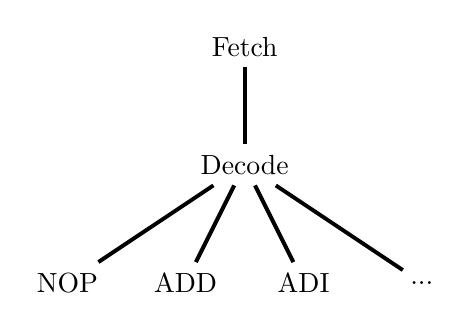
\begin{tikzpicture} [scale=1.00]
  \usepgflibrary{shapes.multipart}
  \usetikzlibrary{trees} 
  % make all path lines (the node shapes) a little thicker
  \tikzstyle{every path}=[line width=0.50mm]  
  
  \node(F0) {Fetch}
    child {node {Decode}
      child {node {NOP}}
      child {node {ADD}}
      child {node {ADI}}
      child {node {...}}
    };
  ;
  \end{tikzpicture}
\end{figure}

The \gls{cpu} designer would continue to design states for all instructions and end each state with a loop back to Fetch in order to get the next instruction out of \gls{ram}.

Designing a \gls{cpu} is no insignificant task and is well beyond the scope of this book. However, one of the labs in the accompanying lab manual design a very simple processor that demonstrates how bits are moved around a circuit based upon control codes.